\documentclass[oneside,final]{article}
\usepackage[T2A]{fontenc}
\usepackage[utf8x]{inputenc}
\usepackage[russian, english]{babel}
\usepackage{vmargin}
\usepackage{graphicx}
\setpapersize{A4}
\setmarginsrb{2cm}{1.5cm}{1cm}{1.5cm}{0pt}{0mm}{0pt}{13mm}
\usepackage{indentfirst}
\usepackage{gensymb}
\usepackage[pdftex,unicode]{hyperref}
\sloppy
\begin{document}
\large
\thispagestyle{empty}
\par \centerline{Московский Государственный Университет им.Л.В.Ломоносова}
\par \centerline{Факультет вычислительной математики и кибернетики}
\vfill
\par \centerline{Отчет по практикуму}
\par \centerline{\textbf{Солнечная система}}
\vfill
\par \rightline{Хартикова Анастасия, 331}
\vfill
\par \centerline{Москва, 2012}
\newpage
\section{Постановка задачи}

\par \textbf{Компьютерная модель Солнечной системы}
\par Изобразить на экране компьютера Солнце и основные тела Солнечной
системы: восемь планет (от Меркурия до Нептуна), их основные спутники
(Луна для Земли, Фобос и Деймос для Марса, Ио, Европа, Ганимед и
Каллисто для Юпитера, Ариель, Оберон для Урана и многие другие),
карликовые планеты (Плутон) в их движении
по
орбитам. Вращение планет вокруг Солнца происходит в
разных плоскостях, однако плоскости орбит планет близки к плоскости
земной орбиты, а карликовая планета Плутон из этой плоскости выбивается.
Вращение
планет вокруг своей оси не учитывается. Также
моделируется следующее астрономическое событие в Солнечной системе: пролет
кометы через Солнечную систему.
\oar Цель моделирования – наблюдение различных конфигураций планет и их
спутников, а также выбранного астрономического события.
\par Моделирование движения планет базируется на известных астрономам 6
величинах - так называемых орбитальных элементах, выведенных из законов
Кеплера. Они полностью определяют орбиту космического объекта, её наклон
по отношению к эклиптике, скорости и положения тела в любой момент
времени. Время отсчитывается от так называемой юлианской эпохи J2000.
Это одна из текущих точек отсчёта, для которой вычислены данные эфемериды.
Единицей измерения времени является юлианское столетие, равное 100
обычным годам. В программе имеется возможность изменять скорость течения
времени, начиная от 1 обычного земного дня.
\par Между тем при визуализации Солнечной системы на экране компьютера
не может быть соблюдено правильное соотношение размеров орбит планет и скоростей
их
движения, т.к. все планеты будут в лучшем случае показаны точками.
Спутники разглядеть будет тем более невозможно. Кометы также не обладают
большим радиусом, а орбиты их громадны. Однако делается попытка сделать
объекты пропорциональными их реальным радиусам. Это достигается разными
коэффициентами масштабирования для внутренних и внешних планет, а также
их спутников.
\par Для улучшения видимости предоставляется скроллинг изображения, а
также возможность поворота плоскости эклиптики вокруг закреплённой точки
- Солнца. Имеется функция отображения названий всех объектов Солнечной
системы по выбору пользователя. На экран также выводятся некоторые
программные данные, как то: время на компьютере пользователя(начальная
точка), время в программе, ускорение течения времени, FPS.
\par Пользователю предоставляется возможность добавлять и удалять объекты
Солнечной системы через конфигурационный xml-файл, без перекомпиляции
программы. Таким образом, можно смоделировать Солнечную систему с любой
желаемой точностью.
\par Программа учитывает разную скорость отрисовки кадров и меняет в
зависимости от FPS скорость течения времени.

\section{Диаграмма классов}
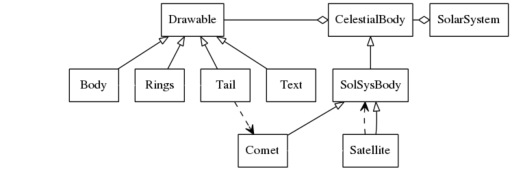
\includegraphics[]{2.png}

\section{Диаграмма объектов}
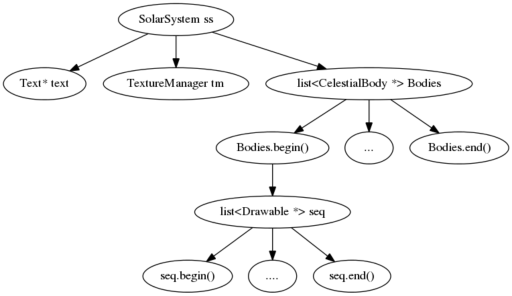
\includegraphics[]{3.png}

\section{Текстовые спецификафии интерфейса основных классов системы}

\begin{verbatim}

// Класс Солнечная система
class SolarSystem
{
public:
    SolarSystem ();
    virtual ~SolarSystem ();
    void init(); // инициализация текста
    void readXML(string filename); // чтение xml-файла
    void parseXML(const xmlpp::Node *node, CelestialBody* p = NULL); // парсинг xml-файла
    void nextFrame(); // пересчёт положений, времени
    void addBody(CelestialBody *p); // добавить тело в систему
    void speedUp(); // ускорить течение времени
    void slowDown(); // замедлить течение времени
    void move(); // включить движение
    void step(); // сделать шаг
    void stop(); // поставить на паузу
    time_t getTime(); 
    double getSpeed();
    Text* getText();
    void setFPS(double fps);
    void setWScale(double WScale);
    void setPrompt(bool prompt);
    void setWIncl(Vector WIncle);

private:
    /* data */
    std::list< CelestialBody* > Bodies; // тела Солнечной системы
    std::set<Glib::ustring> solarTypes; // типы в xml для CelestialBody и его производных
    std::set<Glib::ustring> drawTypes; // типы в xml для Drawable и его производных
    TextureManager tm; 
    Text* text;
    double T; //time
    double delta;
    double delta_delta;
    bool moves, steps;
    double fps;
    double WScale;
    Vector WIncle;
    bool prompt;
};

// Класс Небесное тело. Пример: Солнце.
class CelestialBody
{
public:
    CelestialBody (): scale(0) {};
    virtual ~CelestialBody ();
    void Draw(); // нарисовать объект
    void add(Drawable *object); // добавить фигуру
    void remove(); // удалить фигуру
    void nextFrame(double T); // пересчёт положений
    virtual Vector getPos(double T);
    virtual double getA();
    virtual double getScale() const;
    void setScale(double scale);
    void setText(Text* text);
    void setName(std::string name);

private:
    /* data */
    std::list< Drawable* > seq; // набор фигур
    double scale;
    Text* text;
    std::string name;
};

// Класс Тело солнечной системы. Планеты и карликовые планеты. Примеры: Меркурий-Плутон.
class SolSysBody: public CelestialBody
{
public:
    SolSysBody(double a, double e, double M0, double n, double O, double i, double w);
    virtual ~SolSysBody (){};
    Vector State(double T); // расчёт состояния
    virtual void Kepler(double GM, double M, double T, double a, double e); // расчёт орбиты
    void Ellip(double GM, double M, double a, double e); // для эллиптических орбит
    virtual Vector getPos(double T);
    virtual double getA();
    Vector setPos(Vector vec);
    Vector getVel() const;

private:
    /* data */
    double a, e, M0, O, i, w, n;
    Vector pos;
    Vector r, v; // temp vectors
    double T_last;
};

// Класс Спутник. Примеры: Фобос, Ариель, Оберон.
class Satellite: public SolSysBody
{
public:
    Satellite (double a, double e, double M0, double n, double O, double i, double w): SolSysBody (a, e, M0, n, O, i, w) {};
    virtual ~Satellite () {};
    virtual Vector getPos(double T); // вычисляет положение с учётом планеты
    virtual double getA();
    void setPlanet(SolSysBody* planet); // установить планету, вокруг которой вращается спутник
    double getScale() const;

private:
    /* data */
    SolSysBody* planet;
};

// Класс Комета. Пример: комета Галлея.
class Comet: public SolSysBody
{
public:
    Comet (double a, double e, double M0, double n, double O, double i, double w): SolSysBody (a, e, M0, n, O, i, w) {};
    virtual ~Comet (){};
    void Kepler(double GM, double T0, double T, double q, double e); // переопределённый Кеплер
    void addTail(Tail *tail_new); // добавить хвост
    Vector getPos(double T);

private:
    /* data */
    Tail* tail;
    bool tail_added;
};

// Базовый интерфейс для отрисовки
class Drawable
{
public:
    Drawable (): axis(1, 1, 1), position(0, 0, 0), incl(0, 0, 0), scale(1), angle(0.0f), w(0) {};
    virtual ~Drawable (){};
    void Draw(); // нарисовать
    virtual void DrawObject(){}; // отрисовка конкретного объекта, переопределяется в наследуемых классах.
    void setPos(Vector pos);
    void setScale(double scale);
    void setIncl(Vector incl);

private:
    /* data */
	Vector axis, position, incl;
    double scale, angle, w;
};

// Класс Тело. Рисует сферу.
class Body: public Drawable
{
public:
    Body (double R, GLuint texture);
    virtual ~Body (){};
    void DrawObject();

private:
    /* data */
    GLUquadricObj *sphere;
    double R;
    GLuint texture;
};

// Класс Кольца. Примеры: кольца Сатурна, Урана.
class Rings: public Drawable
{
public:
    Rings (double R1, double R2, GLuint texture);
    virtual ~Rings (){};
    void DrawObject();

private:
    /* data */
    double R1, R2;
    GLuint texture;
    GLuint list;
};

// Класс Текст.
class Text: public Drawable
{
public:
    Text(GLuint texture);
    virtual ~Text ();
    void DrawObject(); // вывести в 3D окружении
    void setText(std::string new_text);
    void print(int x, int y, std::string _text, int W, int H); // напечатать поверх всего лицом к пользователю
    void setWScale(double WScale);
private:
    /* data */
    std::string text;
    GLuint texture;
    GLuint list;
    double WScale;
};

// Класс Хвост кометы.
class Tail: public Drawable
{
public:
    Tail(GLuint texture);
    virtual ~Tail (){};
    void DrawObject();
    void setVel(Vector v){};
private:
    /* data */
    particle particles[MAX_PARTICLES];
    Vector velocity;
    GLuint texture;
    GLuint list;
};
\end{verbatim}

\section{Пользовательский интерфейс}
\subsection{Клавиши управления}
\begin{verbatim}
    Esc - выход из программы
    Space - перейти в режим пошаговой отладки.
    Enter - выйти из режим пошаговой отладки.
    +/- - увеличить/уменьшить масштаб.
    ( и ) - замедлить или ускорить программу.
    t - показать подсказки: имена тел Солнечной системы.
    Мышью при зажатой левой кнопке - повернуть плоскость эклиптики.
\end{verbatim}

\subsection{Скриншоты программы}
\begin{figure}[h!]
    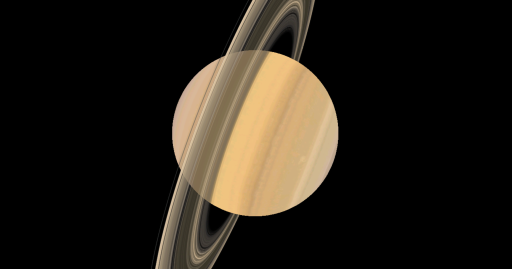
\includegraphics{s1.png}
    \caption{Сатурн и его кольца}
\end{figure}
\begin{figure}[h!]
    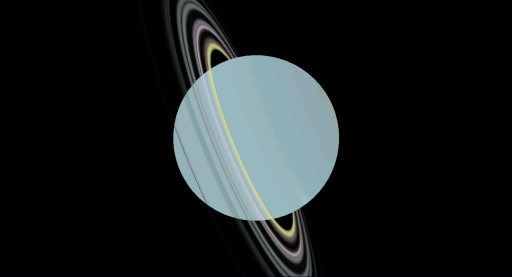
\includegraphics{s2.png}
    \caption{Уран и его кольца}
\end{figure}
\begin{figure}[h!]
    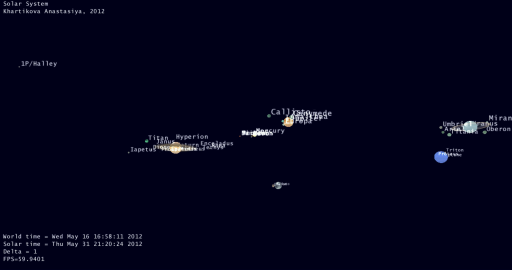
\includegraphics{s3.png}
    \caption{Общий вид программы}
\end{figure}

\section{Инструментальные стредства}
\par Язык разработки: С++
\par Инструменты разработки: vim, gcc, make.
\par Библиотеки: freeglut, glew, xml++.
\par Система контроля версий: git 1.7.10.

\section{Файловая система}
\par SolarSystem.xml - конфигурационный файл Солнечной системы.
\par SolarSystem.cpp, SolarSystem.h -- объявление и реализация класса SolarSystem.
\par CelestialBody.cpp, CelestialBody.h -- объявление и реализация CelestialBody.
\par SolSysBody.cpp, SolSysBody.h -- объявление и реализация классов SolSysBody, Satellite.
\par Comet.cpp, Comet.h -- объявление и реализация класса Comet.
\par Drawable.cpp, Drawable.h -- объявление и реализация классов Drawable, Body, Rings, Tail, Text.
\par TextureManager.cpp, TextureManager.h -- объявление и реализация классов TextureManager и Image.
\par Math.cpp, Math.h -- объявление и реализация классов Vector и Matrix.
\par main.cpp, main.h -- инициализация и обеспечение работы GLUT.
\par Makefile -- файл для сборки.

\end{document}
